\section{Estatística Bayesiana}

\subsection{Leituras Recomendadas}
\begin{frame}{Estatística Bayesiana - Leituras Recomendadas}
	\begin{vfilleditems}
		\item \textcite{gelman2013bayesian} - Capítulo 1: Probability and inference
		\item \textcite{mcelreath2020statistical} - Capítulo 1: The Golem of Prague
		\item \textcite{gelman2020regression} - Capítulo 3: Some basic methods in mathematics and probability
		\item \textcite{khanBayesianLearningRule2021}
		\item \textcite{storopoli2021estatisticabayesianaR} - O que é Estatística Bayesiana?
		\item \textbf{Probabilidade}:
		\begin{vfilleditems}
			\item Um ótimo livro-texto - \textcite{bertsekasIntroductionProbability2nd2008}
			\item Um ótimo livro-texto (pule a parte de estatística frequentista) - \textcite{dekkingModernIntroductionProbability2010}
			\item Do ponto de vista Bayesiano e com abordagem filosófica - \textcite{jaynesProbabilityTheoryLogic2003}
			\item Do ponto de vista Bayesiano e com abordagem simples e lúdica - \textcite{kurtBayesianStatisticsFun2019}
			\item Abordagem filosófica e uma exposição não focada no rigor matemático - \textcite{diaconisTenGreatIdeas2019}
		\end{vfilleditems}
	\end{vfilleditems}
\end{frame}

\subsection{O que é Estatística Bayesiana}
\begin{frame}{O que é Estatística Bayesiana}
	A estatística Bayesiana\footnote{maiúsculo, pois se refere ao teorema de Bayes que é um sobrenome}
	é uma abordagem de análise de dados baseada no teorema de Bayes,
	onde o conhecimento disponível sobre os parâmetros em um modelo estatístico
	é atualizado com as informações dos dados observados
	\parencite{gelman2013bayesian}. O conhecimento prévio é expresso como
	uma distribuição
	\textit{a priori}\footnote{do inglês \foreignlanguage{english}{\textit{prior distribution}}}
	e combinado com os dados observados na forma de uma função de
	verossimilhança\footnote{do inglês \foreignlanguage{english}{\textit{likelihood function}}}
	para determinar a distribuição
	posterior\footnote{\foreignlanguage{english}{do inglês \textit{posterior distribution}}}.
	A posterior também pode ser usada para fazer previsões sobre eventos futuros.
\end{frame}

\subsubsection{O que muda da Estatística Frequentista?}
\begin{frame}{O que muda da Estatística Frequentista?}
	\begin{vfilleditems}
		\item \textbf{Flexibilidade} - peças probabilísticas para construir um modelo\footnote{como se fosse LEGO}:
		\begin{vfilleditems}
			\item Conjecturas probabilísticas sobre os parâmetros:
			\begin{vfilleditems}
				\item \textit{Priori}
				\item Verossimilhança
			\end{vfilleditems}
		\end{vfilleditems}
		\item Melhor tratamento da \textbf{incerteza}:
		\begin{vfilleditems}
			\item Coerência
			\item Propagação
			\item Não se usa \textit{"se amostrássemos infinitamente de uma população que não existe..."}
		\end{vfilleditems}
		\item Sem \textbf{$p$-valores}:
		\begin{vfilleditems}
			\item Todas as intuições estatísticas fazem \textbf{sentido}
			\item 95\% de certeza que o valor do parâmetro $\theta$ está entre $x$ e $y$
			\item Quase \textbf{impossível} fazer $p$-hacking.
		\end{vfilleditems}
	\end{vfilleditems}
\end{frame}

\begin{frame}{Um pouco mais de Formalidade}
	\begin{vfilleditems}
		\item Estatística Bayesiana usa declarações probabilísticas:
		\begin{vfilleditems}
			\item um ou mais parâmetros $\theta$
			\item dados não-observados $\tilde{y}$
		\end{vfilleditems}
		\item Essas declarações são condicionadas nos valores observados de $y$:
		\begin{vfilleditems}
			\item $P(\theta \mid y)$
			\item $P(\tilde{y} \mid y)$
		\end{vfilleditems}
		\item Nós também, de maneira implícita, condicionados nos valores observados de quaisquer co-variáveis $x$
	\end{vfilleditems}
\end{frame}

\begin{frame}{Principal Mudança}
	\begin{defn}[Estatística Bayesiana]
		O uso do Teorema de Bayes\footnote{mais sobre ele já já...} como o procedimento de \textbf{estimativa dos parâmetros de interesse $\theta$ ou dados não-observados $\tilde{y}$}. \parencite{gelman2013bayesian}
	\end{defn}
\end{frame}

\subsection{Ferramentas}

\begin{frame}{Ferramentas para Estatística Bayesiana}
	\begin{vfilleditems}
		\item \LARGE  \href{https://mc-stan.org}{\texttt{Stan}}
		\item \texttt{PyMC}
		\item \small \texttt{JAGS}
		\item \footnotesize \texttt{BUGS}
	\end{vfilleditems}
\end{frame}

\subsubsection{Stan}

\begin{frame}{\href{https://mc-stan.org}{\texttt{Stan}}\footnote{\textcite{carpenterStanProbabilisticProgramming2017}}}
	\begin{columns}
		\begin{column}{0.8\textwidth}
			\begin{vfilleditems}
				\small
				\item Plataforma para modelagem e computação estatística de alto desempenho
				\item Suporte financeiro da \href{https://numfocus.org/}{NUMFocus}:
				\begin{vfilleditems}
					\footnotesize
					\item AWS Amazon
					\item Bloomberg
					\item Microsoft
					\item IBM
					\item RStudio
					\item Facebook
					\item NVIDIA
					\item Netflix
				\end{vfilleditems}
				\small
				\item Linguagem própria, similar à \texttt{C++}
				\item Amostrador \textit{Markov Chain Monte Carlo} (MCMC) em paralelo
			\end{vfilleditems}
		\end{column}
		\begin{column}{0.2\textwidth}
			\centering
			\includegraphics[width=0.6\textwidth]{stan_transparent.png}
		\end{column}
	\end{columns}
\end{frame}

\begin{frame}{\href{https://mc-stan.org}{\texttt{Stan}} na Série Billions\footnote{Se não conseguir assistir \href{https://github.com/storopoli/Estatistica-Bayesiana/blob/master/images/stan_billions_subtitled.mp4?raw=true}{clique aqui} para ver o vídeo no seu navegador} (Temporada 3 Episódio 9)}
	\centering
	\includemedia[
		width=\linewidth,
		height=0.3\linewidth,
		addresource=stan_billions_subtitled.mp4,
		transparent,
		activate=pageopen,
		passcontext,  %show VPlayer's right-click menu
		flashvars={
				source=stan_billions_subtitled.mp4
				&loop=true
				&scaleMode=stretch
			}
	]{\texttt{Stan} na Série Billions}{http://mirrors.ctan.org/macros/latex/contrib/media9/players/VPlayer.swf}
\end{frame}

% \begin{frame}[fragile]{Código \href{https://mc-stan.org}{\texttt{Stan}} versus Fórmulas de \texttt{R}}
%     \begin{lstlisting}[basicstyle=\small, language=Stan]
%     data {
%       int<lower=0> N;
%       vector[N] x1;
%       vector[N] x2;
%       vector[N] y;
%     }
%     parameters {
%       real alpha;
%       vector[2] beta;
%       real<lower=0> sigma;
%     }
%     model {
%       sigma ~ cauchy(0, 2.5);
%       y ~ normal(alpha + beta[1] * x1 + beta[2] * x2, sigma);
%     }
%     \end{lstlisting}
% \end{frame}

% \begin{frame}[fragile]{Código \href{https://mc-stan.org}{\texttt{Stan}} versus Fórmulas de \texttt{R}}
%     \begin{lstlisting}
% stan_glm(y ~ x1 + x2, data = df, family = gaussian())
%     \end{lstlisting}
% \end{frame}

% \begin{frame}{\href{https://mc-stan.org}{\texttt{Stan}}\footnote{foi lançado em 2012} na Scopus\footnote{veja as buscas Scopus nos \hyperlink{appendixscopus}{Slides de Backup no final dessa apresentação}}}
%    \centering
%    \begin{tikzpicture}[ybar]
%         \begin{axis}[
%         xlabel=Ano,ylabel=Uso,
%         x tick label style={rotate=45, /pgf/number format/.cd,
%                             scaled x ticks = false,
%                             set thousands separator={},
%                             fixed}]
%         \addplot [draw=blue, fill=blue] coordinates {
%                 (2012, 6)
%                 (2013, 19)
%                 (2014, 62)
%                 (2015, 113)
%                 (2016, 189)
%                 (2017, 387)
%                 (2018, 671)
%                 (2019, 1045)
%                 (2020, 1538)
%             };
%         \end{axis}
%     \end{tikzpicture}
% \end{frame}

% \begin{frame}{\href{https://mc-stan.org}{\texttt{Stan}}\footnote{baseado no \href{https://breckbaldwin.github.io/ScientificSoftwareImpactMetrics/DeepLearningAndBayesianSoftware.html}{reporte anual do Breck Baldwin para a NUMFocus}}\footnote{veja as buscas Scopus nos \hyperlink{appendixscopus}{Slides de Backup no final dessa apresentação}}}
%    \centering
%    \begin{tikzpicture}[ybar]
%         \begin{axis}[
%         nodes near coords={\pgfmathprintnumber[fixed,precision=3]{\pgfplotspointmeta}},
%         ylabel=Uso, xtick={1,2,3,4},
%         ymax=0.85,
%         ytick={0.1, 0.2, 0.3, 0.4, 0.5, 0.6, 0.7, 0.8},
%         xticklabels={\texttt{TensorFlow}, \texttt{PyTorch}, \texttt{Stan}, \texttt{PyMC}}]
%         \addplot [draw=yellow, fill=yellow] coordinates {
%                 (1, 0.713)};
%         \addplot [draw=green, fill=green] coordinates {
%                 (2, 0.161)};
%         \addplot [draw=blue, fill=blue] coordinates {
%                 (3, 0.108)};
%         \addplot [draw=red, fill=red] coordinates {
%                 (4, 0.0176)};
%         \end{axis}
%     \end{tikzpicture}
% \end{frame}

\subsubsection{R}
\begin{frame}{\texttt{R}}
	\begin{vfilleditems}
		\item R é uma linguagem criada \textbf{por estatísticos para estatísticos}
		\item Possui um vasto \textbf{ecossistema de bibliotecas} e é amplamente usado na \textbf{ciência} e em especial nas \textbf{ciências aplicadas}
		\item Quase toda \textbf{tese maluca} ou \textbf{algoritmo inovador} de Estatística/Probabilidade está no \texttt{CRAN} (Repositório de Pacotes \texttt{R}
		\item Como linguagem de programação é \textbf{horrível}\footnote{consegue ser um pouco menos pior que \texttt{Python}}: Recomendo \href{https://julialang.org/}{\texttt{Julia}}
	\end{vfilleditems}
\end{frame}

\subsubsection{Python}
\begin{frame}{\texttt{Python} e \href{http://docs.pymc.io/}{\texttt{PyMC}}}
	\begin{vfilleditems}
		\item \texttt{Python} consegue ser um pouco melhor que \texttt{R}
		\item Mas tem a "tara"~dos anos 90 de tudo ser \textbf{Orientado à Objetos}
		\item \href{http://docs.pymc.io/}{\texttt{PyMC}} \parencite{pymc3}:
		\begin{vfilleditems}
			\item Uma Biblioteca de Estatística Bayesiana com o seu próprio amostrador \textit{Markov Chain Monte Carlo} (MCMC)
			\item Também com Suporte financeiro da \href{https://numfocus.org/}{NUMFocus}
			\item Amarram o cavalo num barco que afundou há algum tempo: \texttt{Theano}
			\item \texttt{Theano} \textbf{morreu} mas os desenvolvedores do \texttt{PyMC} fizeram um \textit{fork} no projeto e estão usando-o como \textit{backend}
		\end{vfilleditems}
	\end{vfilleditems}
\end{frame}

% \begin{frame}[fragile]{Exemplo de Código \href{http://docs.pymc.io/}{\texttt{PyMC}}}
% \begin{lstlisting}[basicstyle=\small, language=Python]
% with Model() as model:
%     sigma = HalfCauchy("sigma", beta=10, testval=1.0)
%     alpha = Normal("Intercept", 0, sigma=20)
%     beta_1 = Normal("beta_1", 0, sigma=2)
%     beta_2 = Normal("beta_2", 0, sigma=2)

%     likelihood = Normal("y",
%                  mu=alpha + beta_1 * x1 + beta_2 * x2,
%                  sigma=sigma, observed=y)
% \end{lstlisting}
% \end{frame}

\subsubsection{Julia}
\begin{frame}{\href{https://julialang.org/}{\texttt{Julia}} e \href{https://turing.ml}{\texttt{Turing}}}
	\begin{vfilleditems}
		\item \href{https://julialang.org/}{\texttt{Julia}} \parencite{bezanson2017julia} é uma linguagem relativamente nova, lançada pela primeira vez em 2012, que visa ser de \textbf{alto nível} e \textbf{rápida}
		\item Linguagem de tipagem \textbf{dinâmica rápida} que compila \textit{just-in-time} (JIT) em código nativo usando \texttt{LLVM}.
		\item "Roda como \texttt{C}, mas lê como \texttt{Python}"~\parencite{perkelJuliaComeSyntax2019}, o que significa que é extremamente \textbf{rápida}, fácil \textbf{prototipagem} e \textbf{ler/escrever} código.
		\item \textbf{Multi-paradigma}, combinando recursos de programação \textbf{imperativa}, \textbf{funcional} e \textbf{orientada a objetos}.
	\end{vfilleditems}
\end{frame}

\begin{frame}{\href{https://turing.ml}{\texttt{Turing}}}
	\begin{vfilleditems}
		\item \href{https://turing.ml}{\texttt{Turing}} é uma \textbf{Linguagem de Programação Probabilística}\footnote{em inglês \textit{probabilistic programming language} (PPL)} escrita totalmente em \href{https://julialang.org/}{\texttt{Julia}}
		\item Usa \textbf{pacotes} de \href{https://julialang.org/}{\texttt{Julia}} para:
		\begin{vfilleditems}
			\item \textbf{Diferenciação Automática}\footnote{\textit{autodiff}}
			\item \textbf{Distribuições Probabilísticas}
			\item \textbf{Solucionadores de Equações Ordinais}\footnote{\textit{Ordinary Differential Equation Solvers} (ODE)}
			\item \textbf{Redes Neurais} (sendo responsável pela parte "Bayesiana"~da Rede Neural Bayesiana)
		\end{vfilleditems}
	\end{vfilleditems}
\end{frame}

% \begin{frame}[fragile]{Exemplo de Código \href{https://turing.ml}{\texttt{Turing}}\footnote{eu acredito que há muito potencial em \texttt{Julia} e escrevi um \href{https://storopoli.github.io/Bayesian-Julia}{tutorial de Estatística Bayesiana usando \texttt{Julia} e \texttt{Turing}} \parencite{storopoli2021bayesianjulia}}}
%     \begin{lstlisting}[basicstyle=\small, language=Matlab, escapeinside=\{\}]
%         @model linreg({$x_1$}, {$x_2$}, y) = begin
%             {$\alpha$} ~ Normal(0, 20)
%             {$\beta_1$} ~ Normal(0, 2)
%             {$\beta_2$} ~ Normal(0, 2)
%             {$\sigma$} ~ Exponential(1)

%             y .~ Normal({$\alpha$} .+ {$\beta_1$} * {$x_1$} + {$\beta_2$} * {$x_2$}, {$\sigma$})
%         end
%     \end{lstlisting}
% \end{frame}

\subsection{Probabilidade}
\begin{frame}{PROBABILIDADE NÃO EXISTE!\footnote{\textcite{definettiTheoryProbability1974}}}
	\begin{columns}
		\begin{column}{0.8\textwidth}
			\begin{vfilleditems}
				\item Sim, a probabilidade não existe.
				\item Ou melhor, probabilidade como uma quantidade física,
				chance objetiva, \textbf{NÃO existe}
				\item se dispensarmos a questão da chance objetiva \textit{nada se perde}
				\item A matemática do raciocínio indutivo permanece
				\textbf{exatamente a mesma}
			\end{vfilleditems}
		\end{column}
		\begin{column}{0.2\textwidth}
			\centering
			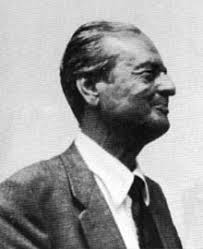
\includegraphics[width=0.9\columnwidth]{finetti.jpg}
		\end{column}
	\end{columns}
\end{frame}

\begin{frame}{PROBABILIDADE NÃO EXISTE!\footnote{\textcite{definettiTheoryProbability1974}}}
	\begin{columns}
		\begin{column}{0.6\textwidth}
			\begin{vfilleditems}
				\small
				\item Considere jogar uma moeda de enviesada
				\item As tentativas são consideradas independentes e, como resultado,
				exibem outra propriedade importante: \textbf{a ordem não importa}
				\item A frequência é considerada uma \textbf{estatística suficiente}
				\item Dizer que a ordem não importa ou dizer que a única coisa que
				importa é a frequência são duas maneiras de dizer exatamente a
				mesma coisa
				\item Dizemos que essa probabilidade é \textbf{invariante sob permutações}
			\end{vfilleditems}
		\end{column}
		\begin{column}{0.4\textwidth}
			\begin{tikzpicture}[
					scale=0.55,
					transform shape, thick,
					every node/.style = {draw, circle, minimum size = 10mm},
					grow = down,  % alignment of characters
					level 1/.style = {sibling distance=3cm},
					level 2/.style = {sibling distance=1.5cm},
					level 3/.style = {sibling distance=3cm},
					level distance = 3cm,
					head/.style = {fill = orange!90!blue,
							label = center:\textsf{\Large C}},
					tail/.style = {fill = blue!70!yellow, text = black,
							label = center:\textsf{\Large K}}
				]
				\node[shape = circle split, draw, line width = 1pt,
					minimum size = 10mm, inner sep = 0mm, font = \sffamily\large,
					rotate=30] (Start)
				{ \rotatebox{-30}{H} \nodepart{lower} \rotatebox{-30}{T}}
				child {   node [head] (A) {}
						child { node [head] (B) {}}
						child { node [tail] (C) {}}
					}
				child {   node [tail] (D) {}
						child { node [head] (E) {}}
						child { node [tail] (F) {}}
					};

				% Filling the root (Start)
				\begin{scope}[on background layer, rotate=30]
					\fill[head] (Start.base) ([xshift = 0mm]Start.east) arc (0:180:5mm)
					-- cycle;
					\fill[tail] (Start.base) ([xshift = 0pt]Start.west) arc (180:360:5mm)
					-- cycle;
				\end{scope}

				% Labels
				\begin{scope}[nodes = {draw = none}]
					\path (Start) -- (A) node [near start, left]  {$0.5$};
					\path (A)     -- (B) node [near start, left]  {$0.5$};
					\path (A)     -- (C) node [near start, right] {$0.5$};
					\path (Start) -- (D) node [near start, right] {$0.5$};
					\path (D)     -- (E) node [near start, left]  {$0.5$};
					\path (D)     -- (F) node [near start, right] {$0.5$};
					\begin{scope}[nodes = {below = 11pt}]
						\node at (B) {$0.25$};
						\node at (C) {$0.25$};
						\node at (E) {$0.25$};
						\node at (F) {$0.25$};
					\end{scope}
				\end{scope}
			\end{tikzpicture}
		\end{column}
	\end{columns}
\end{frame}

\begin{frame}{Interpretações da Probabilidade}
	\begin{vfilleditems}
		\item \textbf{Objetiva} - frequência no longo prazo de um evento específico
		\begin{vfilleditems}
			\item $P(\text{chuva}) = \frac{\text{dias que choveram}}{\text{dias totais}}$
			\item $P(\text{chance de eu ser presidente} = 0)$ (Nunca ocorreu)
		\end{vfilleditems}
		\item \textbf{Subjetiva} - nível de crença em um evento
		\begin{vfilleditems}
			\item $P(\text{chuva}) = \text{crença que choverá}$
			\item $P(\text{chance de eu ser presidente} = 10^{-10})$ (Muito improvável)
		\end{vfilleditems}
	\end{vfilleditems}
\end{frame}

\subsubsection{O que é Probabilidade?}
\begin{frame}{O que é Probabilidade?}
	\begin{defn}[Probabilidade]
		Sobre notação, definimos que $A$ é um evento e $P(A)$ a probabilidade do evento, logo:
		$$
			\{P(A) \in \mathbb{R} : 0 \leq P(A) \leq 1 \}.
		$$
		\vfill
		Isto quer dizer o "probabilidade do evento $A$ ocorrer é o conjunto de
		todos os números reais entre $0$ e $1$; incluindo $0$ e $1$"
	\end{defn}
\end{frame}

\begin{frame}{Axiomas da Probabilidade\footnote{\textcite{kolmogorovFoundationsTheoryProbability1933}}}
	\begin{columns}
		\begin{column}{0.8\textwidth}
			\begin{vfilleditems}
				\item \textbf{Não-negatividade}: Para todo $A$, $P(A) \geq 0$.
				Toda probabilidade é positiva (maior ou igual a zero), independente do
				evento
				\item \textbf{Aditividade}: Para dois \textit{mutuamente exclusivos}
				$A$ e $B$ (não podem ocorrer ao mesmo tempo):
				$P(A) = 1 - P(B)$ e $P(B) = 1 - P(A)$
				\item \textbf{Normalização}: A probabilidade de todos os eventos
				possíveis $A_1, A_2, \dots$ devem somar $1$:
				$\sum_{n \in \mathbb{N}} A_n = 1$
			\end{vfilleditems}
		\end{column}
		\begin{column}{0.2\textwidth}
			\centering
			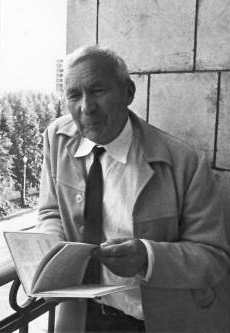
\includegraphics[width=0.9\columnwidth]{kolmogorov.jpg}
		\end{column}
	\end{columns}
\end{frame}

\begin{frame}{Espaços Amostrais}
	\begin{vfilleditems}
		\item Discretos $$\Theta = \left\{1, 2, \ldots, \right\}$$
		\item Contínuos $$\Theta \in \left(-\infty, \infty \right)$$
	\end{vfilleditems}
\end{frame}

\begin{frame}{Espaços Amostrais Discretos}
	8 Planetas do Nosso Sistema Solar
	\begin{vfilleditems}
		\item Mercúrio - $\mercury$
		\item Vênus - $\venus$
		\item Terra - $\earth$
		\item Marte $\mars$
		\item Júpiter - $\jupiter$
		\item Saturno $\saturn$
		\item Urano - $\uranus$
		\item Netuno $\neptune$
	\end{vfilleditems}
\end{frame}

\begin{frame}[fragile]{Espaços Amostrais Discretos\footnote{figuras adaptadas de \href{https://github.com/betanalpha/stan_intro}{Michael Betancourt (CC-BY-SA-4.0)}}}
	\footnotesize
	\begin{figure}
		\centering
		\subfigure{
			\begin{tikzpicture}[scale=0.25, thick]
				\draw[color=black] (-25, 0) to (10, 0);
				\node[] at (-15, 0) {O planeta possui campo magnético};
				\node[] at (7, 2) {$\theta \in E_{1}$};

				\fill[color=gray60] (0, 0) circle (25pt) node[color=black] {$\mercury$};
				\fill[color=blue] (2, 0) circle (25pt) node[color=black] {$\venus$};
				\fill[color=blue] (4, 0) circle (25pt) node[color=black] {$\earth$};
				\fill[color=gray60] (6, 0) circle (25pt) node[color=black] {$\mars$};
				\fill[color=blue] (8, 0) circle (25pt) node[color=black] {$\jupiter$};
				\fill[color=blue] (10, 0) circle (25pt) node[color=black] {$\saturn$};
				\fill[color=blue] (12, 0) circle (25pt) node[color=black] {$\uranus$};
				\fill[color=blue] (14, 0) circle (25pt) node[color=black] {$\neptune$};
			\end{tikzpicture}
		}
		%
		\subfigure{
			\begin{tikzpicture}[scale=0.25, thick]
				\draw[color=black] (-25, 0) to (10, 0);
				\node[] at (-15, 0) {O planeta possui luas};
				\node[] at (7, 2) {$\theta \in E_{2}$};

				\fill[color=gray60] (0, 0) circle (25pt) node[color=black] {$\mercury$};
				\fill[color=gray60] (2, 0) circle (25pt) node[color=black] {$\venus$};
				\fill[color=blue] (4, 0) circle (25pt) node[color=black] {$\earth$};
				\fill[color=blue] (6, 0) circle (25pt) node[color=black] {$\mars$};
				\fill[color=blue] (8, 0) circle (25pt) node[color=black] {$\jupiter$};
				\fill[color=blue] (10, 0) circle (25pt) node[color=black] {$\saturn$};
				\fill[color=blue] (12, 0) circle (25pt) node[color=black] {$\uranus$};
				\fill[color=blue] (14, 0) circle (25pt) node[color=black] {$\neptune$};
			\end{tikzpicture}
		}
		%
		\subfigure{
			\begin{tikzpicture}[scale=0.25, thick]
				\draw[color=black] (-25, 0) to (10, 0);
				\node[] at (-15, 0) {O planeta possui campo magnético e luas};
				\node[] at (7, 2) {$\theta \in E_{1} \cap E_{2}$};

				\fill[color=gray60] (0, 0) circle (25pt) node[color=black] {$\mercury$};
				\fill[color=gray60] (2, 0) circle (25pt) node[color=black] {$\venus$};
				\fill[color=blue] (4, 0) circle (25pt) node[color=black] {$\earth$};
				\fill[color=gray60] (6, 0) circle (25pt) node[color=black] {$\mars$};
				\fill[color=blue] (8, 0) circle (25pt) node[color=black] {$\jupiter$};
				\fill[color=blue] (10, 0) circle (25pt) node[color=black] {$\saturn$};
				\fill[color=blue] (12, 0) circle (25pt) node[color=black] {$\uranus$};
				\fill[color=blue] (14, 0) circle (25pt) node[color=black] {$\neptune$};
			\end{tikzpicture}
		}
		%
		\subfigure{
			\begin{tikzpicture}[scale=0.25, thick]
				\node[] at (-15, 0) {O planeta possui campo magnético ou luas};
				\node[] at (7, 2) {$\theta \in E_{1} \cup E_{2}$};

				\fill[color=gray60] (0, 0) circle (25pt) node[color=black] {$\mercury$};
				\fill[color=blue] (2, 0) circle (25pt) node[color=black] {$\venus$};
				\fill[color=blue] (4, 0) circle (25pt) node[color=black] {$\earth$};
				\fill[color=blue] (6, 0) circle (25pt) node[color=black] {$\mars$};
				\fill[color=blue] (8, 0) circle (25pt) node[color=black] {$\jupiter$};
				\fill[color=blue] (10, 0) circle (25pt) node[color=black] {$\saturn$};
				\fill[color=blue] (12, 0) circle (25pt) node[color=black] {$\uranus$};
				\fill[color=blue] (14, 0) circle (25pt) node[color=black] {$\neptune$};
			\end{tikzpicture}
		}
		%
		\subfigure{
			\begin{tikzpicture}[scale=0.25, thick]
				\node[] at (-15, 0) {O planeta não possui um campo magnético};
				\node[] at (7, 2) {$\theta \in \neg E_{1}$};

				\fill[color=blue] (0, 0) circle (25pt) node[color=black] {$\mercury$};
				\fill[color=gray60] (2, 0) circle (25pt) node[color=black] {$\venus$};
				\fill[color=gray60] (4, 0) circle (25pt) node[color=black] {$\earth$};
				\fill[color=blue] (6, 0) circle (25pt) node[color=black] {$\mars$};
				\fill[color=gray60] (8, 0) circle (25pt) node[color=black] {$\jupiter$};
				\fill[color=gray60] (10, 0) circle (25pt) node[color=black] {$\saturn$};
				\fill[color=gray60] (12, 0) circle (25pt) node[color=black] {$\uranus$};
				\fill[color=gray60] (14, 0) circle (25pt) node[color=black] {$\neptune$};
			\end{tikzpicture}
		}
		%
	\end{figure}
\end{frame}

\begin{frame}{Espaços Amostrais Contínuos\footnote{figuras adaptadas de \href{https://github.com/betanalpha/stan_intro}{Michael Betancourt (CC-BY-SA-4.0)}}}
	\footnotesize
	\begin{figure}
		\centering
		\subfigure{
			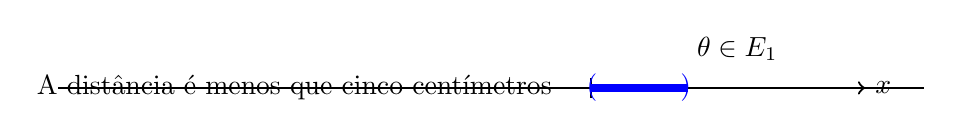
\begin{tikzpicture}[scale=0.25, thick]
				\draw[color=black] (-27, 0) to (17, 0);
				\node[align=center] at (-15, 0) {A distância é menos que cinco centímetros};
				\node[] at (7.5, 2) {$\theta \in E_{1}$};

				\draw[|->] (0, 0) -- (14,0) node[right] {$x$};
				\draw[line width=1mm, color=blue] (0, 0) node[] {$\,($} -- (5, 0) node[] {$\!)$};
			\end{tikzpicture}
		}
		%
		\subfigure{
			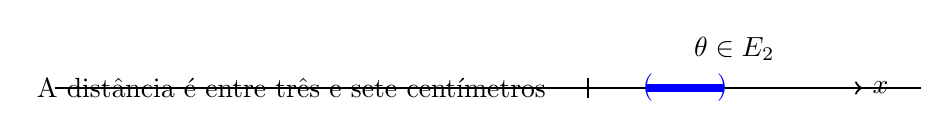
\begin{tikzpicture}[scale=0.25, thick]
				\draw[color=black] (-27, 0) to (17, 0);
				\node[align=center] at (-15, 0) {A distância é entre três e sete centímetros};
				\node[] at (7.5, 2) {$\theta \in E_{2}$};

				\draw[|->] (0, 0) -- (14,0) node[right] {$x$};
				\draw[line width=1mm, color=blue] (3, 0) node[] {$\,($} -- (7,0) node[] {$\!)$};

			\end{tikzpicture}
		}
		%
		\subfigure{
			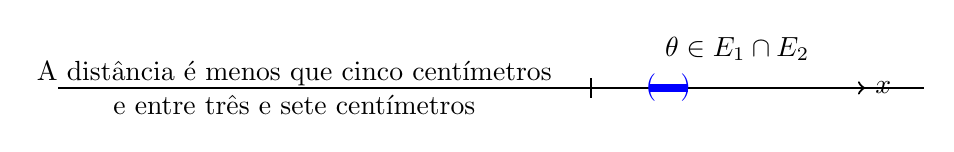
\begin{tikzpicture}[scale=0.25, thick]
				\draw[color=black] (-27, 0) to (17, 0);
				\node[align=center] at (-15, 0) {A distância é menos que cinco centímetros \\ e entre três e sete centímetros};
				\node[] at (7.5, 2) {$\theta \in E_{1} \cap E_{2}$};

				\draw[|->] (0, 0) -- (14,0) node[right] {$x$};
				\draw[line width=1mm, color=blue] (3, 0) node[] {$\,($} -- (5, 0) node[] {$\!)$};
			\end{tikzpicture}
		}
		%
		\subfigure{
			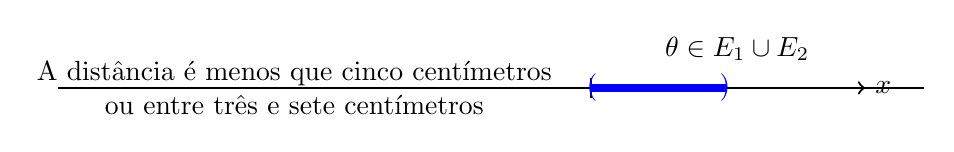
\begin{tikzpicture}[scale=0.25, thick]
				\draw[color=black] (-27, 0) to (17, 0);
				\node[align=center] at (-15, 0) {A distância é menos que cinco centímetros \\ ou entre três e sete centímetros};
				\node[] at (7.5, 2) {$\theta \in E_{1} \cup E_{2}$};

				\draw[|->] (0, 0) -- (14, 0) node[right] {$x$};
				\draw[line width=1mm, color=blue] (0, 0) node[] {$\,($} -- (7, 0) node[] {$\!)$};
			\end{tikzpicture}
		}
		%
		\subfigure{
			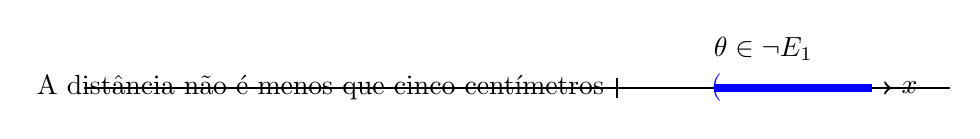
\begin{tikzpicture}[scale=0.25, thick]
				\draw[color=black] (-27, 0) to (17, 0);
				\node[align=center] at (-15, 0) {A distância não é menos que cinco centímetros};
				\node[] at (7.5, 2) {$\theta \in \neg E_{1}$};

				\draw[|->] (0, 0) -- (14, 0) node[right] {$x$};
				\draw[line width=1mm, color=blue] (5, 0) node[] {$\,($} -- (13, 0);
			\end{tikzpicture}
		}
	\end{figure}
\end{frame}

\begin{frame}{Parâmetros Discretos versus Contínuos}

	Tudo o que foi exposto até agora partiu do pressuposto que os parâmetros
	são discretos. Isto foi feito com o intuito de prover uma melhor intuição
	do que é probabilidade. Nem sempre trabalhamos com parâmetros discretos.
	Os parâmetros podem ser contínuos, como por exemplo: idade, altura, peso etc.
	Mas não se desespere, todas as regras e axiomas da probabilidade são válidos
	também para parâmetros contínuos. A única coisa que temos que fazer é trocar
	todas as somas $\sum$ por integrais $\int$. Por exemplo o terceiro axioma de
	\textbf{Normalização} para variáveis aleatórias contínuas se torna:

	$$
		\int_{x \in X} p(x) dx = 1.
	$$

\end{frame}


\begin{frame}{Probabilidade Condicional}
	\begin{defn}[Probabilidade Condicional]
		Probabilidade de um evento ocorrer caso outro tenha ocorrido ou não. \newline \newline
		A notação que usamos é $P( A \mid B )$, que lê-se como "a probabilidade
		de observamos $A$ dado que já observamos $B$". \newline \newline
		\vfill \vfill
		$$
			\begin{aligned}
				P(A \mid B) & = \frac{\text{número de elementos em $A$ e $B$}}{\text{número de elemementos em $B$}} \\
				P(A \mid B) & = \frac{P(A \cap B)}{(B)}
			\end{aligned}
		$$
		\newline \newline \hspace{0.7\textwidth}
		{\footnotesize assumimos que $P(B) > 0$}.
	\end{defn}
\end{frame}

\begin{frame}{Exemplo de Probabilidade Condicional}
	\begin{exemplo}[Poker Texas Hold'em]
		\begin{vfilleditems}
			\item \textbf{Espaço Amostral}: $52$ cartas no baralho, $13$ tipos de cartas e $4$ tipos de naipes.
			\item $P(A)$: Chance de receber um Ás $\left( \frac{4}{52} = \frac{1}{13}\right)$
			\item $P(K)$: Chance de receber um Rei (K) $\left( \frac{4}{52} = \frac{1}{13} \right)$
			\item $P(A \mid K)$: Chance de receber um Ás, dado que você recebeu um Rei (K) $\left( \frac{4}{51} \approx 0.078 \right)$
			\item $P(K \mid A)$: Chance de receber um Rei (K), dado que você recebeu um Ás $\left( \frac{4}{51} \approx 0.078 \right)$
		\end{vfilleditems}
	\end{exemplo}
\end{frame}

\begin{frame}{Cuidado! Nem sempre $P(A \mid B) = P(B \mid A)$}
	No exemplo anterior temos a simetria $P(A \mid K) = P(K \mid A)$, \textbf{mas nem sempre isso é verdade}\footnote{Mais especificamente, se as taxas basais $P(A)$ e $P(B)$ não são iguais, a simetria é quebrada $P(A \mid B) \neq P(B \mid A)$!}
	\begin{exemplo}[O Papa é católico]
		\begin{vfilleditems}
			\small{
				\item $P(\text{papa})$: Chance alguém aleatório ser papa, algo bem pequeno, 1 em 8 bilhões $\left( \frac{1}{8 \cdot 10^9} \right)$
				\item $P(\text{católico})$: Chance alguém aleatório ser católico, 1.34 de 8 bilhões $\left( \frac{1.34}{8} \approx 0.17 \right)$
				\item $P(\text{católico} \mid \text{papa})$: Chance do Papa ser católico $\left( \frac{999}{1000} = 0.999 \right)$
				\item $P(\text{papa} \mid \text{católico})$: Chance de alguém católico ser o papa $\left( \frac{1}{1.34 \cdot 10^9} \cdot 0.999 \approx 7.46 \cdot 10^{-10} \right)$
			}
			\item \large{\textbf{Logo}: $P(\text{católico} \mid \text{papa}) \neq P(\text{papa} \mid \text{católico})$}
		\end{vfilleditems}
	\end{exemplo}
\end{frame}

\begin{frame}{Um clássico da Probabilidade}
	\begin{columns}
		\begin{column}{0.6\textwidth}
			\begin{exemplo}[Monty Hall]
				\begin{vfilleditems}
					\small
					\item Um apresentador de TV lhe apresenta 3 portas
					\item Uma delas tem um prêmio: um carro! As outras tem um bode
					\item Você deve escolher uma porta (que não é aberta)
					\item Nesse momento Monty abre uma das outras duas portas que você
					não escolheu, revelando que o carro não se encontra nessa porta e revelando um dos bodes
					\item Monty então lhe pergunta "Você quer manter sua escolha de porta ou trocar?"
				\end{vfilleditems}
			\end{exemplo}
		\end{column}
		\begin{column}{0.4\textwidth}
			\begin{figure}
				\centering
				\def\svgwidth{\columnwidth}
				\input{../images/monty_hall.pdf_tex}
			\end{figure}
		\end{column}
	\end{columns}
\end{frame}

\begin{frame}{Solução do Problema de Monty Hall}
	\begin{idea}[Probabilidade de ganhar o carro]
		$$
			\begin{aligned}
				P(\text{carro} \mid C_i) & = \frac{1}{3}                                                                                                                          \\
				P(\text{carro})          & = \frac{1}{3} \cdot P(\text{carro} \mid C_1) + \frac{1}{3} \cdot P(\text{carro} \mid C_2) + \frac{1}{3} \cdot P(\text{carro} \mid C_3) \\
				P(\text{carro})          & = \frac{\sum^3_{i=1}P(\text{carro} \mid C_i)}{3}                                                                                       \\
				P(\text{carro})          & = \frac{1}{3}
			\end{aligned}
		$$
	\end{idea}
	\vfill \vfill
	$C_i$ é o evento no qual o carro está atrás da porta $i$, $i=1,2,3$
\end{frame}

\begin{frame}[t]{Solução do Problema de Monty Hall\footnote{se você não acredita nesse resultado veja como simular o problema de Monty Hall nos \hyperlink{appendixmontyhall}{Slides de Backup no final dessa apresentação}}}
	\begin{columns}[t]
		\begin{column}{0.5\textwidth}
			{\Large \textbf{Cenário 1}: Não trocar de porta} \newline \newline
			Simples: $$\frac{1}{3}$$
		\end{column}
		\begin{column}{0.5\textwidth}
			{\Large \textbf{Cenário 2}: Trocar de porta} \newline \newline
			Escolha qualquer porta $i$ para ser $C_i = 0$
			\vfill
			$$
				\begin{aligned}
					P(\text{carro}) & = 0 \cdot P(\text{carro} \mid C_i) + \frac{1}{3} + \frac{1}{3} \\
					P(\text{carro}) & = \frac{2}{3}
				\end{aligned}
			$$
		\end{column}
	\end{columns}
\end{frame}

\begin{frame}{Visualização do Problema de Monty Hall}
	\begin{figure}
		\centering
		\subfigure{
			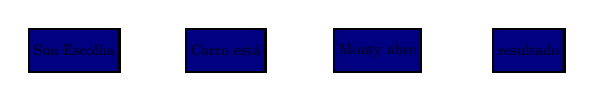
\begin{tikzpicture}[
					scale=0.55,
					header/.style = {draw, rectangle, fill = blue!50!black, minimum size = 10mm},
					level distance = 3.5cm,
					transform shape, thick,
					grow = right, sloped,
				]
				\node[header] {Sua Escolha}
				child{
						node[header] {Carro está}
						edge from parent[draw=none]
						child{
								node[header] {Monty abre}
								edge from parent[draw=none]
								child{
										node[header] {resultado}
										edge from parent[draw=none]
									}
							}
					};
			\end{tikzpicture}
		}
		%
		\subfigure{
			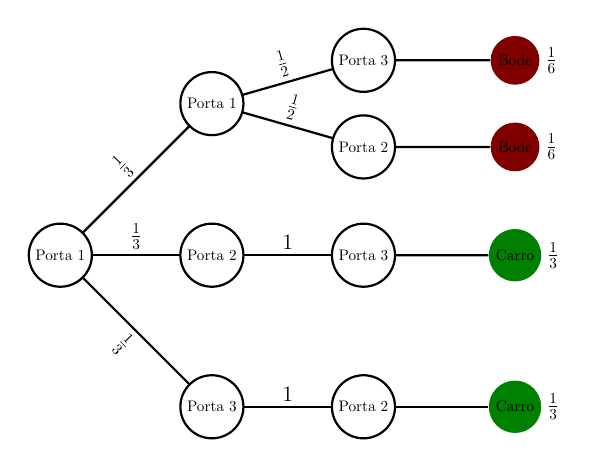
\begin{tikzpicture}[
					scale=0.55,
					door/.style = {draw, circle, minimum size = 10mm},
					car/.style = {circle, fill = green!50!black, minimum size = 10mm},
					goat/.style = {circle, fill = red!50!black, minimum size = 10mm},
					level distance = 3.5cm,
					transform shape, thick,
					grow = right, sloped,
					level 1/.style = {sibling distance=3.5cm},
					level 2/.style = {sibling distance=2cm},
					level 3/.style = {sibling distance=3cm}
				]
				\node[door] {Porta 1}
				child {
				node[door] {Porta 3}
				child {
				node[door] {Porta 2}
				child {
				node[car, label=right:{\Large$\frac{1}{3}$}] {Carro}
				}
				edge from parent
				node[above] {\Large$1$}
				}
				edge from parent
				node[below] {\Large$\frac{1}{3}$}
				}
				child {
				node[door] {Porta 2}
				child {
				node[door] {Porta 3}
				child {
				node[car, label=right:{\Large$\frac{1}{3}$}] {Carro}
				}
				edge from parent
				node[above] {\Large$1$}
				}
				edge from parent
				node[above] {\Large$\frac{1}{3}$}
				}
				child {
				node[door] {Porta 1}
				child {
				node[door] {Porta 2}
				child {
				node[goat, label=right:{\Large$\frac{1}{6}$}] {Bode}
				}
				edge from parent
				node[above]  {\Large$\frac{1}{2}$}
				}
				child {
				node[door] {Porta 3}
				child {
				node[goat, label=right:{\Large$\frac{1}{6}$}] {Bode}
				}
				edge from parent
				node[above]  {\Large$\frac{1}{2}$}
				}
				edge from parent
				node[above] {\Large$\frac{1}{3}$}
				};
			\end{tikzpicture}
		}
	\end{figure}
\end{frame}

\begin{frame}{Probabilidade Conjunta}
	\begin{defn}[Probabilidade Conjunta]
		Probabilidade de observados dois ou mais eventos ocorrem. \newline \newline
		A notação que usamos é $P(A, B)$, que lê-se como
		"a probabilidade de observamos $A$ e também observamos $B$". \newline \newline
		$$
			\begin{aligned}
				P(A,B) & = \text{número de elementos em $A$ ou $B$} \\
				P(A,B) & = P(A \cup B)
			\end{aligned}
		$$
	\end{defn}
\end{frame}

\begin{frame}{Exemplo de Probabilidade Conjunta}
	\begin{exemplo}[Revisitando Poker Texas Hold'em]
		\begin{vfilleditems}
			{\footnotesize
				\item \textbf{Espaço Amostral}: $52$ cartas no baralho, $13$ tipos de cartas e $4$ tipos de naipes.
				\item $P(A)$: Chance de receber um Ás $\left( \frac{4}{52} = \frac{1}{13}\right)$
				\item $P(K)$: Chance de receber um Rei (K) $\left( \frac{4}{52} = \frac{1}{13} \right)$
				\item $P(A \mid K)$: Chance de receber um Ás, dado que você recebeu um Rei (K) $\left( \frac{4}{51} \approx 0.078 \right)$
				\item $P(K \mid A)$: Chance de receber um Rei (K), dado que você recebeu um Ás $\left( \frac{4}{51} \approx 0.078 \right)$
			}
			\item $P(A, K)$: Chance de receber um Ás e um Rei (K)
			$$
				\begin{aligned}
					P(A, K)                         & = P(K, A)                         \\
					P(A) \cdot P(K \mid A)          & = P(K) \cdot P(A \mid K)          \\
					\frac{1}{13} \cdot \frac{4}{51} & = \frac{1}{13} \cdot \frac{4}{51} \\
					                                & \approx 0.006
				\end{aligned}
			$$
		\end{vfilleditems}
	\end{exemplo}
\end{frame}

% Exemplo do Poker com pacote pst-poker
% Exemplo do Papa e Católico

% Bivariate Normal inspirada aqui: https://github.com/walmes/Tikz/blob/master/src/bivariate-normal.pgf
\begin{frame}{Visualização de Probabilidade Conjunta vs Probabilidade Condicional}
	\centering
	\begin{tikzpicture}[scale=0.9]
		\begin{axis}[
				domain   = -3.5:3.5,
				domain y = -3.5:3.5,
				view = {-70}{20},
				title={$P(X,Y)$ versus $P(X \mid Y=-0.75)$},
				xlabel={$X$},
				ylabel={$Y$},
				% zlabel={$SSE(\beta_0, \beta_1)$},
				zmin = -0,
				%xticklabels=\empty,
				%yticklabels=\empty,
				zticklabels=\empty,
				xtick=\empty,
				ytick={-0.75},
				ztick=\empty,
				axis z line*=none,
				axis y line*=left,
				axis x line*= bottom]
			\addplot3 [
				domain = -3.5:3.5,
				samples = 50, samples y = 0,
				thick, smooth, color = red, fill = orange, opacity = 0.75]
			(x, -0.75, {conditionalbinormal(-0.75, 0, 1, 0, 1, 0.75)});

			\draw (-3.5, -0.75, 0) -- (3.5, -0.75, 0);

			\addplot3 [
				surf,
				domain = -3.5:3.5,
				samples = 50,
				opacity = 0.15,
				faceted color = colorB,
				colormap = {blueblack}{
						color = (colorB)
						color = (colorA!50!white)
						color = (colorA)}]
			{binormal(0, 1, 0, 1, 0.7)};
		\end{axis}
	\end{tikzpicture}
\end{frame}

% Countour plot inspirado daqui: https://tex.stackexchange.com/a/31713/200209
\begin{frame}{Visualização de Probabilidade Conjunta vs Probabilidade Condicional}
	\begin{columns}
		\begin{column}{0.5\textwidth}
			\centering
			\begin{tikzpicture}[scale=0.5]
				\begin{axis}[
						view={0}{90},
						axis equal,
						enlarge y limits=true,
						title={$P(X,Y)$},
						xlabel={$X$},
						ylabel={$Y$},
						xtick=\empty,
						ytick={-0.75}
					]

					\draw[red, line width=2pt] (-3.5, -0.75) -- (3.5, -0.75);

					\addplot3[contour gnuplot={labels=false},domain=-3.5:3.5,domain y=-3.5:3.5]
					{exp(-( x^2 + y^2)/3 )};

				\end{axis}
			\end{tikzpicture}
		\end{column}
		\begin{column}{0.5\textwidth}
			\centering
			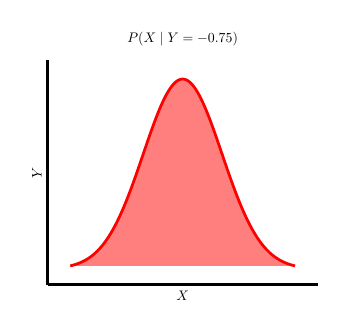
\begin{tikzpicture}[scale=0.5]
				\begin{axis}[every axis plot, line width=2pt,
						title={$P(X \mid Y=-0.75)$},
						xlabel={$X$},
						ylabel={$Y$},
						xtick=\empty,
						ytick=\empty,
						domain=-3.5:3.5,samples=200,
						axis x line*=bottom, % no box around the plot, only x and y axis
						axis y line*=left, % the * suppresses the arrow tips
						enlarge x limits=true
					] % extend the axes a bit

					\addplot [red, fill = red, fill opacity = 0.5] {exp(-( x^2 + -0.75^2)/3 )};
				\end{axis}
			\end{tikzpicture}
		\end{column}
	\end{columns}
\end{frame}

\subsubsection{Teorema de Bayes}
\begin{frame}{Quem foi Thomas Bayes?}
	\begin{columns}
		\begin{column}{0.8\textwidth}
			\begin{vfilleditems}
				\item \small Thomas Bayes (1701 - 1761) foi um estatístico, filósofo
				e ministro presbiteriano inglês conhecido por formular um caso
				específico do teorema que leva seu nome
				\item \small Bayes nunca publicou o que se tornaria sua realização mais famosa;
				suas notas foram editadas e publicadas após sua morte pelo seu amigo
				Richard Price
				\item \small O nome formal do teorema é Bayes-Price-Laplace, pois Thomas
				Bayes foi o primeiro a descobrir, Richard Price pegou seus rascunhos,
				formalizou em notação matemática e apresentou para a Royal Society of London,
				e Pierre Laplace redescobriu o teorema sem ter tido contato prévio no final
				do século XVIII na França ao usar probabilidade para inferência estatística
				com dados do Censo na era Napoleônica
			\end{vfilleditems}
		\end{column}
		\begin{column}{0.2\textwidth}
			\centering
			\includegraphics[width=0.9\columnwidth]{thomas_bayes.png}
		\end{column}
	\end{columns}
\end{frame}


\begin{frame}{Teorema de Bayes}
	\begin{theo}[Bayes]
		Nos diz como "inverter" a probabilidade condicional: \newline \newline
		$$P(A \mid B) = \frac{P(A) \cdot P(B \mid A)}{P(B)}$$
	\end{theo}
\end{frame}

\begin{frame}{Prova do Teorema de Bayes}
	Lembra que temos a seguinte identidade na probabilidade:
	$$
		\begin{aligned}
			P(A,B)                 & = P(B,A)                 \\
			P(A) \cdot P(B \mid A) & = P(B) \cdot P(A \mid B)
		\end{aligned}
	$$

	Pois bem, agora passe o $P(B)$ do lado direito para o lado esquerdo dividindo:
	$$
		\begin{aligned}
			P(A) \cdot P(B \mid A)              & = \overbrace{P(B)}^{\text{isso vai para $\leftarrow$}} \cdot \quad P(A \mid B) \\
			                                    &                                                                                \\
			\frac{P(A) \cdot P(B \mid A)}{P(B)} & = P(A \mid B)                                                                  \\
			P(A \mid B)                         & = \frac{P(A) \cdot P(B \mid A)}{P(B)}
		\end{aligned}
	$$
\end{frame}

\begin{frame}{Visualização do Teorema de Bayes}
	\begin{columns}
		\begin{column}{0.6\textwidth}
			\begin{tikzpicture}[thick]
				\node[circle, label={137:Espaço Amostral}, fill=red!20!white, fill opacity = 0.5, minimum size=6cm] (Omega) at (0,0) {};
				\node[ellipse, label={35:$E_1$}, fill=blue, fill opacity = 0.5, minimum width=5.5cm, minimum height=2cm] (Ellipse) at (0,1) {};
				\node[circle, label={178:$E_2$}, fill=red, fill opacity = 0.5, minimum size = 1cm] (Circulo) at (-1.5,1) {};
				\node[] (KK) at (-1.5, 1) {$KK$};
				\node[] (CC) at (1.5, 1) {$CC$};
				\node[] (KC) at (1.5, -1) {$KC$};
				\node[] (CK) at (-1.5, -1) {$CK$};
			\end{tikzpicture}
		\end{column}
		\begin{column}{0.4\textwidth}
			$$
				\begin{aligned}
					E_1 & = P(KK  \cup CC) \\
					E_2 & = P(KK \mid E_1)
				\end{aligned}
			$$
		\end{column}
	\end{columns}
\end{frame}

\begin{frame}{Mais um clássico da Probabilidade\footnote{Origem: \href{https://www.yudkowsky.net/rational/bayes}{Yudkowski - \textit{An Intuitive Explanation of Bayes’ Theorem}}}}
	\begin{exemplo}[Cancêr de Mama]
		\small
		O quão acurado é o teste de \textbf{câncer de mama}?
		\begin{vfilleditems}
			\item \footnotesize 1\% das mulheres têm \textbf{câncer de mama} (Prevalência)
			\item \footnotesize 80\% das mamografias detectam o \textbf{câncer de mama} (Verdadeiro Positivo)
			\item \footnotesize 9.6\% das mamografias detectam \textbf{câncer de mama} quando não há incidência (Falso Positivo)
		\end{vfilleditems}
		$$
			\begin{aligned}
				P(C \mid +) & = \frac{P(+ \mid C) \cdot P(C)}{P(+)}                                                      \\
				P(C \mid +) & = \frac{P(+ \mid C) \cdot P(C)}{P(+ \mid C) \cdot P(C) + P(+ \mid \neg C) \cdot P(\neg C)} \\
				P(C \mid +) & = \frac{0.8 \cdot 0.01}{0.8 \cdot 0.01 + 0.096 \cdot 0.99}                                 \\
				P(C \mid +) & \approx 0.0776
			\end{aligned}
		$$
	\end{exemplo}
\end{frame}


\begin{frame}{Porquê o teorema de Bayes é Importante?}
	\begin{idea}[Podemos Inverter a Probabilidade Condicional]
		$$
			\begin{aligned}
				P(\text{hipótese} \mid \text{dados}) = \frac{P(\text{hipótese}) \cdot P(\text{dados} \mid \text{hipótese})}{P(\text{data})}
			\end{aligned}
		$$
	\end{idea}
	Mas isso não é o $p$-valor? \textcolor{red}{\textbf{NÃO!}}
\end{frame}

\subsection{Estatística Frequentista versus Bayesiana}
\subsubsection{O que são $p$-valores e Intervalos de Confiança}
\begin{frame}{O que é o $p$-valor?}
	\begin{defn}[$p$-valor]
		$p$-valor é a probabilidade de obter resultados no mínimo tão
		extremos quanto os que foram observados, dado que a hipótese nula
		$H_0$ é verdadeira
		$$P(D \mid H_0)$$
	\end{defn}
\end{frame}

\begin{frame}{O que \textbf{não é} o $p$-valor!}
	\centering
	\includegraphics[width=0.7\textwidth]{meme-pvalue.jpg}
\end{frame}

\begin{frame}{O que \textbf{não é} o $p$-valor!}
	\begin{vfilleditems}
		\item \textbf{$p$-valor não é a probabilidade da Hipótese nula}
		- Famosa confusão entre $P(D \mid H_0)$ e $P(H_0 \mid D)$.
		Para obter a $P(H_0 \mid D)$ você precisa de estatística Bayesiana.
		\item \textbf{$p$-valor não é a probabilidade dos dados serem produzidos pelo acaso}
		- \textcolor{red}{Não!} Ninguém falou nada de acaso.
		\item \textbf{$p$-valor mensura o tamanho do efeito de um teste estatístico}
		- Também \textcolor{red}{não}... $p$-valor não diz nada sobre o tamanho do efeito.
		Apenas sobre se o quanto os dados observados divergem do esperado sob a hipótese nula.
		Além disso, $p$-valores podem ser "hackeados" de diversas maneiras \parencite{head2015extent}.
	\end{vfilleditems}
\end{frame}

\begin{frame}{A relação entre $p$-valor e $H_0$}
	Para descobrir o $p$-valor, \textbf{descubra a $H_0$ que está por trás dele}.
	Sua definição nunca mudará, pois ela sempre é $P(D \mid H_0)$:
	\begin{vfilleditems}
		\item \textbf{Teste $t$}: $P(D \mid \text{a diferença entre os grupos é zero})$
		\item \textbf{ANOVA}: $P(D \mid \text{não há diferença entre os grupos})$
		\item \textbf{Regressão}: $P(D \mid \text{coeficiente é nulo})$
		\item \textbf{Shapiro-Wilk}: $P(D \mid \text{população é distribuída como uma normal})$
	\end{vfilleditems}
\end{frame}

\begin{frame}{O que são Intervalos de Confiança?}
	\begin{columns}
		\begin{column}{0.8\textwidth}
			\begin{defn}[Intervalos de Confiança]
				\begin{quotation}
					Um intervalo de confiança de X\% para um parâmetro é um intervalo
					$(a, b)$ gerado por um procedimento que em amostragem repetida
					tem uma probabilidade de X\% de conter o valor verdadeiro do
					parâmetro, para todos os valores possíveis do parâmetro
				\end{quotation}
				\vfill \vfill
				\textcite{neyman1937outline} (o "pai" dos intervalos de confiança)
			\end{defn}
		\end{column}
		\begin{column}{0.2\textwidth}
			\centering
			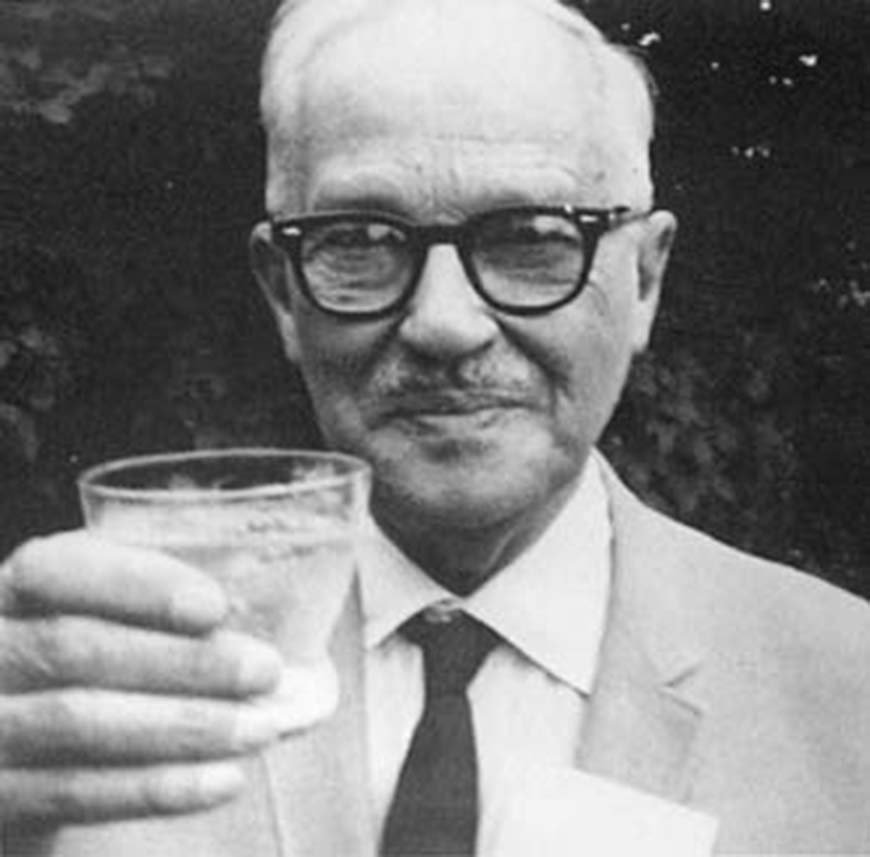
\includegraphics[width=0.9\columnwidth]{neyman.jpeg}
		\end{column}
	\end{columns}
\end{frame}

\begin{frame}{O que são Intervalos de Confiança?}
	\begin{exemplo}[Intervalo de Confiança de uma Política Pública]
		Digamos que você executou uma análise estatística para comparar
		eficácia de uma política pública em dois grupos e você obteve a
		diferença entre a média desses grupos. Você pode expressar essa
		diferença como um intervalo de confiança. Geralmente escolhemos a
		confiança de 95\%. Isso quer dizer que \textbf{95 estudos de 100},
		que usem o \textbf{mesmo tamanho de amostra e população-alvo},
		aplicando o \textbf{mesmo teste estatístico}, esperarão encontrar
		um resultado de diferenças de média entre grupos entre o intervalo
		de confiança.
	\end{exemplo}
	\footnotesize \textcolor{red}{Não diz nada sobre a sua \textbf{população-alvo},
		mas sim sobre a sua \textbf{amostra} num processo maluco de \textbf{amostragem infinita}...}
\end{frame}

\begin{frame}{Intevalos de Confiança versus Intervalos da Posterior}
	\centering
	\begin{tikzpicture}
		\begin{axis}[every axis plot, line width=2pt,
				xmin=0, xmax=4,
				ymin=0, ymax=1.5,
				ylabel=\empty,
				xlabel={$\theta$},
				samples=200,
				axis x line*=bottom, % no box around the plot, only x and y axis
				axis y line*=left,
				enlarge x limits=true,
			] % extend the axes a bit

			\addplot [blue, domain=0:4, forget plot] {lognormal(0, 2)};
			\addplot+ [
				mark=none,
				area legend,
				line width=0pt,
				color=blue,
				fill=blue, fill opacity=0.5,
				domain=0.25950495026507125:3.8534910373715427
			]
			{lognormal(0, 2)} \closedcycle;
			\addlegendentry{50\% Posterior}
			\addplot[red, mark=none] (-0.09, 1.4739034450607542) to (0.09, 1.4739034450607542);
			\addlegendentry{MLE}
			\draw [red] (0,0) to (0, 1.4739034450607542);
		\end{axis}
	\end{tikzpicture}
\end{frame}

\begin{frame}{Intevalos de Confiança versus Intervalos da Posterior}
	\centering
	\begin{tikzpicture}
		\begin{axis}[every axis plot, line width=2pt,
				xmin=-3, xmax=14,
				%ymin=0, ymax=1.5,
				ylabel=\empty,
				xlabel={$\theta$},
				samples=200,
				axis x line*=bottom, % no box around the plot, only x and y axis
				axis y line*=left,
				enlarge x limits=true,
				%legend pos=outer north east, %there is one default value for the `legend pos' that is outside the axis
				%legend cell align=left, % so the legend looks a bit better
			] % extend the axes a bit

			\addplot [blue, domain=-3:14, forget plot] {sumtwonormals(2, 1, 0.6, 10, 1, 0.4)};
			\addplot+ [
				mark=none,
				area legend,
				line width=0pt,
				color=blue,
				fill=blue, fill opacity=0.5,
				domain=1.8:9.7
			]
			{sumtwonormals(2, 1, 0.6, 10, 1, 0.4)} \closedcycle;
			\addlegendentry{50\% Posterior}
			\addplot[red, mark=none] (1.5, 0.24) to (2.5, 0.24);
			\addlegendentry{MLE}
			\draw [red] (2,0) to (2, 0.24);
		\end{axis}
	\end{tikzpicture}
\end{frame}

\begin{frame}{Mas por quê eu nunca vejo estatística sem $p$-valor?}
	\begin{columns}
		\begin{column}{0.8\textwidth}
			Não tem como entendermos $p$-valores se não compreendermos as suas
			origens e trajetória histórica. A primeira menção do termo foi feita
			pelo estatístico Ronald Fisher em 1925 \parencite{fisher1925statistical}:
			\begin{quotation}
				[$p$-valor é] índice que mede a força da evidência contra a hipótese nula
			\end{quotation}
			\begin{vfilleditems}
				\item Para quantificar a força da evidência contra a hipótese nula, Fisher defendeu
				"$p<0.05$ como um nível padrão para concluir que há evidência contra a hipótese testada"
				\item "Não seremos frequentemente perdidos se traçarmos uma linha convencional de 0.05"
			\end{vfilleditems}
		\end{column}
		\begin{column}{0.2\textwidth}
			\centering
			\includegraphics[width=0.9\columnwidth]{fisher.jpg}
		\end{column}
	\end{columns}
\end{frame}

\begin{frame}{$p = 0.06$}
	\begin{vfilleditems}
		\item Como o $p$-valor é uma probabilidade, ele é uma quantidade contínua.
		\item Não há razão para diferenciarmos um $p$ de 0.049 contra um $p$ de 0.051.
		\item Robert Rosenthal, um psicólogo já dizia "Deus ama $p$ de 0.06 tanto quanto um $p$ de 0.05"~\parencite{rosnow1989statistical}.
	\end{vfilleditems}
\end{frame}

\begin{frame}{Mas por quê eu nunca ouvi falar de Estatística Bayesiana?\footnote{\textit{inverse probability} é como o teorema de Bayes era chamado no começo do século XX}}
	\begin{columns}
		\begin{column}{0.8\textwidth}
			\begin{quotation}
				… it will be sufficient … to reaffirm my personal conviction …
				that the theory of inverse probability is founded upon an error,
				and must be wholly rejected.
			\end{quotation}
			\vfill \vfill
			\textcite{fisher1925statistical}
		\end{column}
		\begin{column}{0.2\textwidth}
			\centering
			\includegraphics[width=0.9\columnwidth]{fisher.jpg}
		\end{column}
	\end{columns}
\end{frame}

\begin{frame}{Dentro de todo não Bayesiano há um Bayesiano querendo sair\footnote{Dennis Lindley "Inside every nonBayesian there is a Bayesian struggling to get out"}}
	\begin{columns}
		\begin{column}{0.8\textwidth}
			\begin{vfilleditems}
				\item No último ano de sua vida, Fisher publicou um artigo \parencite{fisherExamplesBayesMethod1962} examinando as possibilidades dos métodos Bayesianos, mas com as probabilidades a \textit{priori} a serem determinadas experimentalmente.
				\item Inclusive alguns autores especulam \parencite{jaynesProbabilityTheoryLogic2003} que se Fisher estivesse vivo hoje, ele provavelmente seria um "Bayesiano".
			\end{vfilleditems}
		\end{column}
		\begin{column}{0.2\textwidth}
			\centering
			\includegraphics[width=0.9\columnwidth]{fisher.jpg}
		\end{column}
	\end{columns}
\end{frame}

\subsection{Estatística Bayesiana}
\begin{frame}{Teorema de Bayes como Motor de Inferência}
	\footnotesize Agora que você já sabe o que é probabilidade e o que é o teorema de Bayes, vou propor o seguinte modelo:
	$$
		\underbrace{P(\theta \mid y)}_{\text{Posterior}} = \frac{\overbrace{P(y \mid  \theta)}^{\text{Verossimilhança}} \cdot \overbrace{P(\theta)}^{\textit{Priori}}}{\underbrace{P(y)}_{\text{Constante Normalizadora}}}
	$$
	\begin{vfilleditems}
		\item \footnotesize $\theta$ -- parâmetro(s) de interesse
		\item \footnotesize $y$ -- dados observados
		\item \footnotesize \textbf{\textit{Priori}}: probabilidade prévia do valor do(s) parâmetro(s)
		\item \footnotesize \textbf{Verossimilhança}: probabilidade dos dados observados condicionados aos valores do(s) parâmetro(s)
		\item \footnotesize \textbf{Posterior}: probabilidade posterior do valor do(s) parâmetros após observamos os dados $y$
		\item \footnotesize \textbf{Constante Normalizadora}: $P(y)$ não faz sentido intuitivo. Essa probabilidade é transformada e pode ser interepretada como algo que existe apenas para que o resultado de $P(y \mid \theta) P(\theta)$ seja algo entre 0 e 1 -- uma probabilidade válida.
	\end{vfilleditems}
\end{frame}

\begin{frame}{Teorema de Bayes como Motor de Inferência}
	A estatísica Bayesiana nos permite \textbf{quantificar diretamente a incerteza}
	relacionada ao valor de um ou mais parâmetros do nosso modelo condicionado aos
	dados observados. Isso é a \textbf{característica principal} da estatística
	Bayesiana. Pois estamos estimando diretamente $P(\theta \mid y)$ por meio do
	teorema de Bayes. A estimativa resultante é totalmente intuitiva:
	simplesmente quantifica a intercerteza que temos sobre o valor de um ou mais
	parâmetro condicionado nos dados, nos pressupostos do nosso modelo
	(verossimilhança) e na probabilidade prévia que temos sobre tais valores.
\end{frame}

\subsubsection{Vantagens da Estatísca Bayesiana}
\begin{frame}{Estatística Bayesiana vs Frequentista}
	%\begin{table}[h!]
	\small
	\begin{tabular}{|l|p{.3\textwidth}|p{.3\textwidth}|}
		\toprule
		                       & \textcolor{blue}{\textbf{Estatística Bayesiana}} & \textcolor{red}{\textbf{Estatística Frequentista}}                  \\ \midrule
		\textbf{Dados}         & Fixos –- Não Aleatórios                          & Incertos –- Aleatórios                                              \\ \midrule
		\textbf{Parâmetros}    & Incertos –- Aleatórios                           & Fixos –- Não Aleatórios                                             \\ \midrule
		\textbf{Inferência}    & Incerteza sobre o valor do parâmetro             & Incerteza sobre um processo de amostragem de uma população infinita \\ \midrule
		\textbf{Probabilidade} & Subjetiva                                        & Objetiva (mas com diversos pressupostos dos modelos)                \\ \midrule
		\textbf{Incerteza}     & Intervalo de Credibilidade –- $P(\theta \mid y)$ & Intervalo de Confiança –- $P(y \mid \theta)$                        \\
		\bottomrule
	\end{tabular}
	%\end{table}
\end{frame}

\begin{frame}{Vantagens da Estatística Bayesiana}
	\begin{vfilleditems}
		\item Abordagem Natural para expressar Incerteza
		\item Habilidade de incorporar Informações Prévias
		\item Maior Flexibilidade do Modelo
		\item Distribuição Posterior completa dos Parâmetros
		\item Propagação Natural da Incerteza
	\end{vfilleditems}
	\small \textbf{Principal Desvantagem}: Velocidade lenta de estimativa de modelos\footnote{\textit{e.g.} 30 segundos ao invés de 3 segundos na abordagem frequentista}
\end{frame}

\begin{frame}{O começo do fim da Estatística Frequentista}
	\begin{vfilleditems}
		\small
		\item Saiba que você está em um momento da história no qual a Estatística está passando por grandes mudanças
		\item Acredito que a estatística frequentista, em especial a maneira que qualificamos evidências e hipóteses
		com $p$-valores se transformará de maneira "significante".
		\item Há cinco anos atrás, a \textit{American Statistical Association} (ASA) publicou uma declaração sobre
		$p$-valores \parencite{Wasserstein2016}. A declaração diz exatamente o que falamos aqui: Os conceitos principais do teste de significância de hipótese nula e, em particular $p$-valores não conseguem prover o que os pesquisadores requerem deles. Apesar do que dizem muitos livros de estatística, materiais de ensinos e artigos publicados, $p$-valores abaixo de 0,05 não "provam" a realidade de nada. Nem, chegando a esse ponto, os $p$-valores acima de 0,05 refutam alguma coisa.
		\item A declaração da ASA tem mais de 3.600 citações provocando impacto relevante.
	\end{vfilleditems}
\end{frame}

\begin{frame}{O começo do fim da Estatística Frequentista}
	\begin{vfilleditems}
		\small
		\item Um simpósio internacional foi promovido em 2017 que originou uma edição especial de acesso aberto da
		\textit{The American Statistician} dedicada à maneiras práticas de abandonarmos $p < 0.05$
		\parencite{wassersteinMovingWorld052019}.
		\item Logo na sequência vieram mais tentativas e reivindicações.
		Em setembro de 2017, a \textit{Nature Human Behaviour} publicou um editorial propondo que o nível de
		significância do $p$-valor seja reduzido de $0.05$ para $0.005$ \parencite{benjaminRedefineStatisticalSignificance2018}
		Diversos autores, inclusive muitos estatísticos altamente influentes e importantes argumentaram que esse simples passo
		ajudaria a combater o problema da crise de replicabilidade da ciência, que muitos acreditam ser a principal
		consequência do uso abusivo de $p$-valores \parencite{Ioannidis2019}.
		\item Além disso, muitos foram um passo além e sugerem que a ciência descarte de uma vez por todas $p$-valores
		\parencite{ItTimeTalk2019,lakensJustifyYourAlpha2018}. Muitos sugerem (eu inclusive) que a principal ferramenta
		de inferência seja a estatística Bayesiana \parencite{amrheinScientistsRiseStatistical2019, Goodman1180, vandeschootBayesianStatisticsModelling2021}
	\end{vfilleditems}
\end{frame}
